% !TEX root =../LibroTipoETSI.tex
%El anterior comando permite compilar este documento llamando al documento raíz
\chapter{Introducción}\label{chp-02}

%\lettrine[lraise=-0.1, lines=2, loversize=0.2]{E}{n} la robótica, uno de los mayores problemas es la percepción del entorno y su ubicación en él. En concreto, cuando se habla de vehículos aéreos no tripulados (UAV), suelen poder posicionarse en el exterior con una precisión de metros. Sin embargo, cuando se trata de navegar en interiores o con precisión más alta el coste de los componentes puede ser muy elevados. Por ejemplo, en exteriores, se puede utilizar la \textit{navegación cinética satelital en tiempo real} (RTK) o en interiores se pueden utilizar balizas acústicas.


%%%%%%%%%%%%%%%%%%%%%%%
\lettrine[lraise=-0.1, lines=2, loversize=0.2]{A}{ctualmente}, los vehículos autónomos no están al alcance de cualquiera. Estos no deben de confundirse con los vehículos no tripulados, como los UAVs (Vehículos aéreos no tripulados) que si están más extendidos, llegando a utilizarse para ocio o para negocios estando al alcance del bosillo de cada vez más gente. La mayoría tienen una autonomía parcial y necesitan la supervisión de un piloto en algunas de sus fases de vuelo, como por ejemplo en el aterrizaje o cuando se navega cerca de obstáculos. Además muchos de ellos solo pueden volar en exteriores donde le llega la señal de los satélites. 
La causa de todas estás limitaciones está en que no pueden determinar dónde están ubicados con exactitud y que la precisión que sulelen tener es de varios metros. Si se mejorase ese aspecto, el número de aplicaciones en las que se podría utilizar sería enorme. 
Por ejemplo, se podría programar un vuelo de reconocimiento cuando se detecte un intruso en una propiedad. También perimitiría manipular objetos como la recogida y depósito de paquetes.  

% Autonomo permite:
% - que no tengan experiencia
% - que se pueda activar las 24 horas del día sin nadie pendiente
% - que sea escalable
% - Si existe una base es más inmediato
El interés de realizar estas tareas de forma autónoma no solo está en que cualquiera pueda hacer uso del vehículo, sin necesitar licencia ni habilidades especiales, si no que también hace el sistema más escalable. Si se quisiera por ejemplo, instalar un sistema de reparto de paquetes mediante vehículos aéreos, y la flota es cada vez más grande, llegará un momento que sea dificil que todos los pilotos se pongan de acuerdo compartiendo el mismo espácio aéreo. Si esta planificación la hace en su lugar un ordenador, posiblemente el sistema sea más optimo. Como última ventaja de la automatización se podría decir que el vehículo podría estar disponible de forma inmediata en cualquier momento y no obligaría a las personas a estar trabajando en horas de descanso. 

%Existen formas pero son más caras:
Si se disponen de los suficientes recursos existe la tecnología para conseguirlo, por ejemplo mediante balizas sonoras, que son usadas en interiores de fábricas o si se opera en el exterior, existe la posibilidad de  \textit{navegación cinética satelital en tiempo real} (RTK). Otra solución que no necesita de instalación en el entorno, son las cámaras o lídares, que con el uso de unos algoritmos llamados SLAM, pueden crear un mapa del entorno y ubicarse en él. El problema de estos es que o bien sus sensores son caros o bien tienen una alta carga computacional que obligan a instalar grandes y costosos ordenadores a bordo del vehículo. 

\begin{figure}[b]
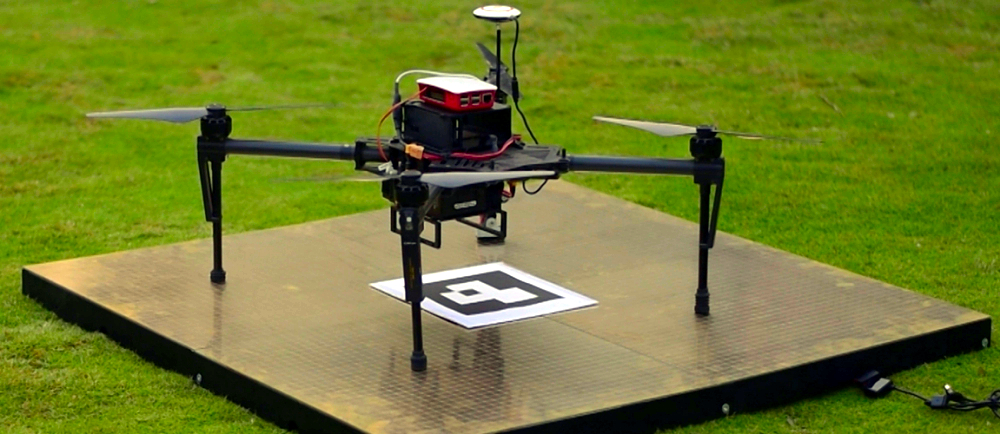
\includegraphics[width=0.7\textwidth]{introduccion/flytbase_en.jpg}
\caption{Estación de carga de \textit{Flytbase}}
\label{fig:flyt}
\end{figure}

%La alternativa: marcadores visuales
Lo que se busca en este trabajo es una alternativa más barata que consiga un posicionamiento centimétrico del vehículo. En concreto se ha hecho uso de unos marcadores visuales planos. Estos contienen figuras que son fácilmente detectables procesando una imagen de dicho marcador, por ejemplo los contornos de un cuadrilátero. Además, para su procesamiento se usará uno de los ordenadores embebidos más baratos del mercado 
% facil de imprimir, requiere menos computo, puede llegar a ser muy robusto. 
% Marcadores visuales. Solución robusta (no hay muchos falsos positivos) ya que es complicado encontrarse en el entorno algo parecido (no como los que usan una pelota), y además barata ya que tiene poco costo computacional, al contrario que los SLAM por ejemplo. 

 
% Implementaciones comerciales
Ya están a la venta algunas soluciones que utilizan esta tecnología para el aterrizaje automático. En concreto algunas  empresas como \textit{Everdrone} \cite{everdrone} y \textit{Flytbase} (ver figura \ref{fig:flyt}) ofrecen estaciones de carga con los mismos marcadores utilizados aquí. 

% Papers
Existen articulos en los que ya han utilizado marcadores visuales para mejorar el posicionamiento de un UAV, la mayoría teniendo como objetivo el aterrizaje automático. En \cite{sani2017automatic} se consigue que un quadrotor \textit{Parrot AR.Drone} aterrice sobre un marcador Aruco, incluso si brevemente se pierde la vista al marcador utilizando las medidas de la IMU. En \cite{yang2015precise} además de la IMU, se utiliza un sensor de flujo óptico para conseguir aterrizar el vehículo. En ninguno de los dos trabajos se utiliza un autopiloto de código abierto, sino se limitan a utilizar las interfaces de programación que aportan Parrot y DJI respectivamente para tomar las medidas de los sensores y comandarle una postura de referencia. 
Además, la falta de detalles de implementación que suele haber en este tipo de artículos, hace que su trabajo sea más dificil de ser repetido por el lector.
En este proyecto, lo que se quiere aportar otro enfoque en el que se hace uso del estimador de estados del autopiloto, el mismo que se utiliza para estimar la orientación y al que le llegan las medidas de la IMU, magnetómetro, barómetro, etc., para obtener una fuente precisa de posición.  
%Esa fusión de las medidas se realiza en el mismo autopiloto, y no en un ordenador externo, con la idea de que los retrasos en las comunicaciones tengan menor efecto. 

% Los puntos que se veran
En este trabajo en primer lugar, en el capítulo \ref{chp:est} se hace un estudio de una parte clave para el posicionamiento con marcadores, que es el estimador de estados. Además se elabora y se muestran los resultados de una simulación en la que se pone a prueba este. En el capítulo \ref{chp:pos} se explica cómo se ha implementado este posicionamiento, mostrando los componentes utilizados y explicando el programa creado. Finalmente, en ese mismo capítulo se enseñan los resultados experimentales a los que se ha llegado.  



\endinput
